% Appendix for eggholder meta-weighting benchmark (unroll=1 only).
\chapter{Meta-weighting benchmark on \texttt{eggholder} (unroll = 1)}
\label{app:meta-weighting-eggholder-u1}

\section{Purpose and scope}

This appendix summarizes the reduced meta-weighting benchmark executed after the
longer differentiable unroll variants (\texttt{meta\_unroll\_steps}=3,5)
showed frequent optimization divergence. To obtain a stable comparison set, the
benchmark was rerun with \texttt{meta\_unroll\_steps}=1 only.

The objective of this experiment was to test whether adaptive gradient-based
loss weighting over Gaussian-continuation targets can improve the final hard
validation loss on the \texttt{eggholder} surface, and under which learning-rate
and noise settings this happens.

\section{Experimental protocol}

\textbf{Benchmark id:} \texttt{meta\_weighting\_eggholder\_u1\_20260504\_221357}.\\
\textbf{Function:} \texttt{eggholder}.\\
\textbf{Completed runs:} 288/288.\\
\textbf{Failed runs:} 0/288.\\
\textbf{Meta lookahead:} \texttt{meta\_unroll\_steps}=1.

\paragraph{Factorial design.}
\begin{itemize}
    \item Numbers of losses: \texttt{1, 2, 3, 5}
    \item Model learning rates: \texttt{0.01, 0.03}
    \item Meta learning rates: \texttt{0.0003, 0.001, 0.003}
    \item Noise ratios: \texttt{0.0, 0.05, 0.2}
    \item Seeds: \texttt{42, 666, 777, 888}
\end{itemize}

Total runs:
\[
4 \times 2 \times 3 \times 3 \times 4 = 288.
\]

\paragraph{Primary metric.}
The main comparison metric is the final hard validation loss
(\texttt{final\_val\_loss}); lower values are better.

\section{Headline results}

\begin{table}[h]
\centering
\small
\begin{tabular}{lrrrr}
\toprule
Losses & Runs & Mean final val loss & Median final val loss & Mean rank \\
\midrule
1 & 72 & 80650.90 & 82870.60 & 2.35 \\
2 & 72 & 81910.62 & 84069.00 & 2.50 \\
3 & 72 & 80974.89 & 82975.01 & 2.43 \\
5 & 72 & 82428.87 & 84139.55 & 2.72 \\
\bottomrule
\end{tabular}
\caption{Aggregate performance by number of weighted losses. Lower validation loss and lower rank are better.}
\label{tab:meta-eggholder-u1-by-losses}
\end{table}

\begin{table}[h]
\centering
\small
\begin{tabular}{lrrr}
\toprule
Losses & Mean improvement vs baseline & Median improvement vs baseline & Fraction improved vs baseline \\
\midrule
2 & -1259.72 & -1089.23 & 0.458 \\
3 &  -324.00 &  -549.98 & 0.472 \\
5 & -1777.98 & -1305.75 & 0.417 \\
\bottomrule
\end{tabular}
\caption{Paired comparison against the baseline \texttt{num\_losses=1}. Positive improvement means that adaptive weighting improves over the baseline; in this experiment all means remain negative.}
\label{tab:meta-eggholder-u1-vs-baseline}
\end{table}

\paragraph{Main takeaway.}
On average, the single-loss baseline (hard-target-only, \texttt{num\_losses=1})
remains the strongest setting in this benchmark. Among the adaptive variants,
\texttt{num\_losses=3} is the closest to the baseline on average, while
\texttt{num\_losses=5} is the weakest overall.

\section{Best observed configurations}

\begin{table}[h]
\centering
\small
\begin{tabular}{lrrrrr}
\toprule
Losses & Noise & $\eta_{\mathrm{model}}$ & $\eta_{\mathrm{meta}}$ & Median final val loss & Mean rank \\
\midrule
1 & 0.00 & 0.03 & 0.0003 & 62717.65 & 1.50 \\
3 & 0.00 & 0.03 & 0.0010 & 69440.03 & 1.75 \\
5 & 0.05 & 0.03 & 0.0030 & 73375.20 & 2.25 \\
3 & 0.05 & 0.03 & 0.0030 & 75490.82 & 2.00 \\
2 & 0.20 & 0.03 & 0.0030 & 75883.22 & 1.75 \\
\bottomrule
\end{tabular}
\caption{Best aggregate settings (sorted approximately by median final validation loss).}
\label{tab:meta-eggholder-u1-best-settings}
\end{table}

The best \emph{single run} in the full matrix was:
\begin{quote}
\texttt{num\_losses=2}, noise ratio \texttt{0.05},
$\eta_{\mathrm{model}}=0.03$, $\eta_{\mathrm{meta}}=0.003$,
seed \texttt{42}, with final validation loss \texttt{52323.09}.
\end{quote}

This means that adaptive weighting can occasionally produce very strong
individual runs, but this advantage was not stable enough across seeds and
conditions to outperform the single-loss baseline on average.

\section{Aggregate visual diagnostics}

\begin{figure}[h]
    \centering
    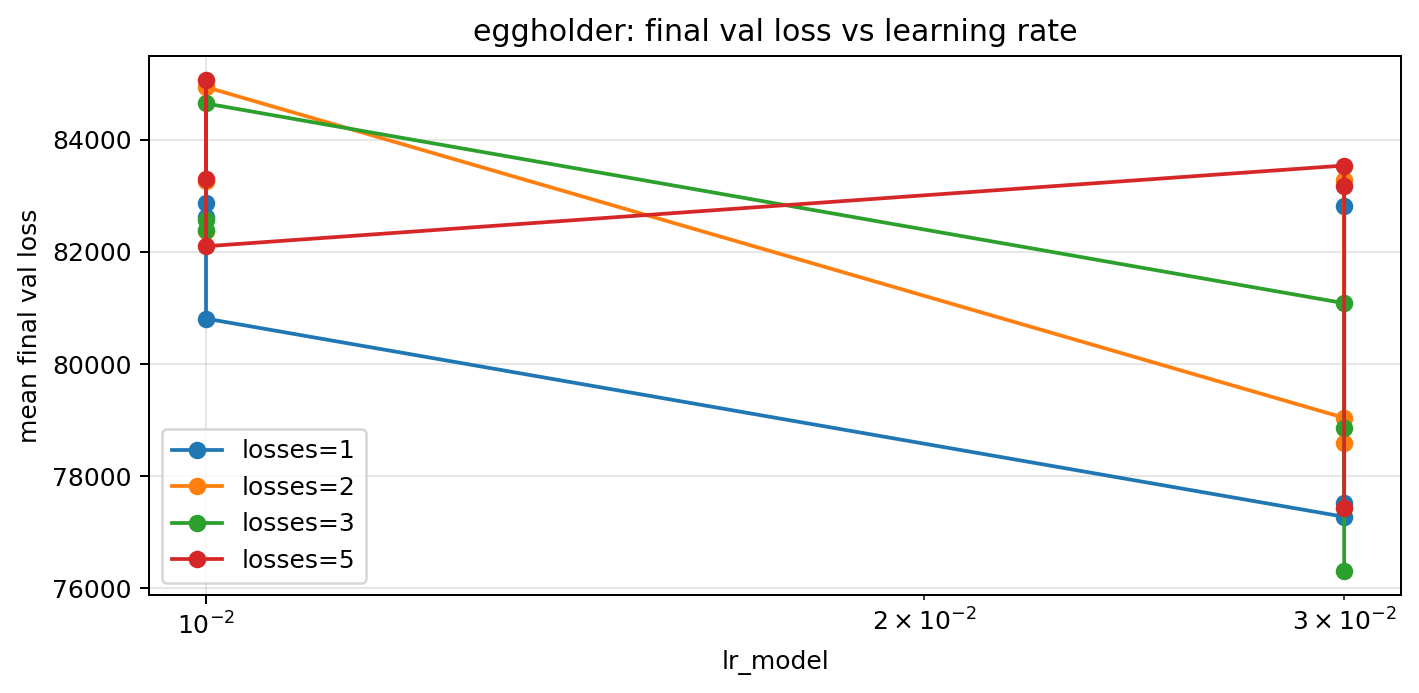
\includegraphics[width=0.92\textwidth]{figures/meta_weighting_eggholder_u1_final_val_loss_vs_lr.png}
    \caption{Mean final validation loss as a function of model learning rate, separated by the number of losses. The higher model learning rate (0.03) is frequently competitive or better than 0.01.}
    \label{fig:meta-eggholder-u1-vs-lr}
\end{figure}

\begin{figure}[h]
    \centering
    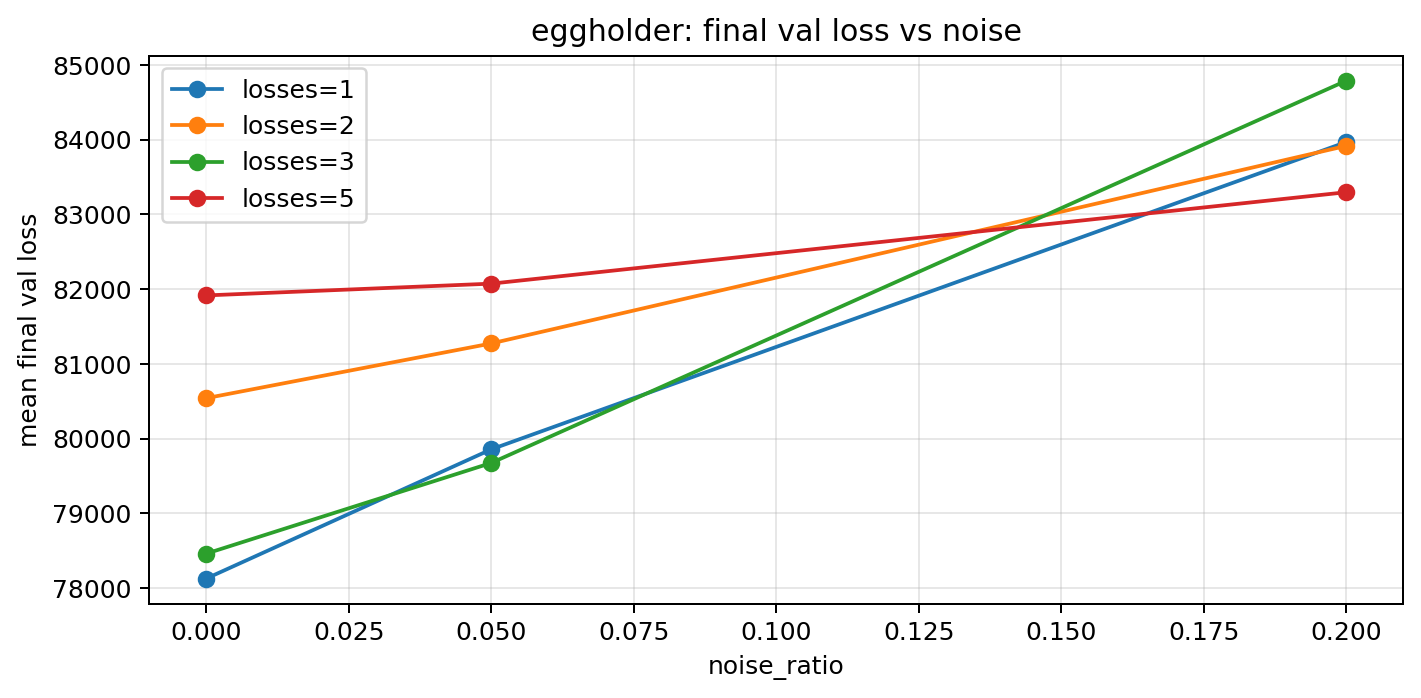
\includegraphics[width=0.92\textwidth]{figures/meta_weighting_eggholder_u1_final_val_loss_vs_noise.png}
    \caption{Mean final validation loss versus noise ratio. Performance generally degrades as noise increases, although the sensitivity depends on the number of losses.}
    \label{fig:meta-eggholder-u1-vs-noise}
\end{figure}

\begin{figure}[h]
    \centering
    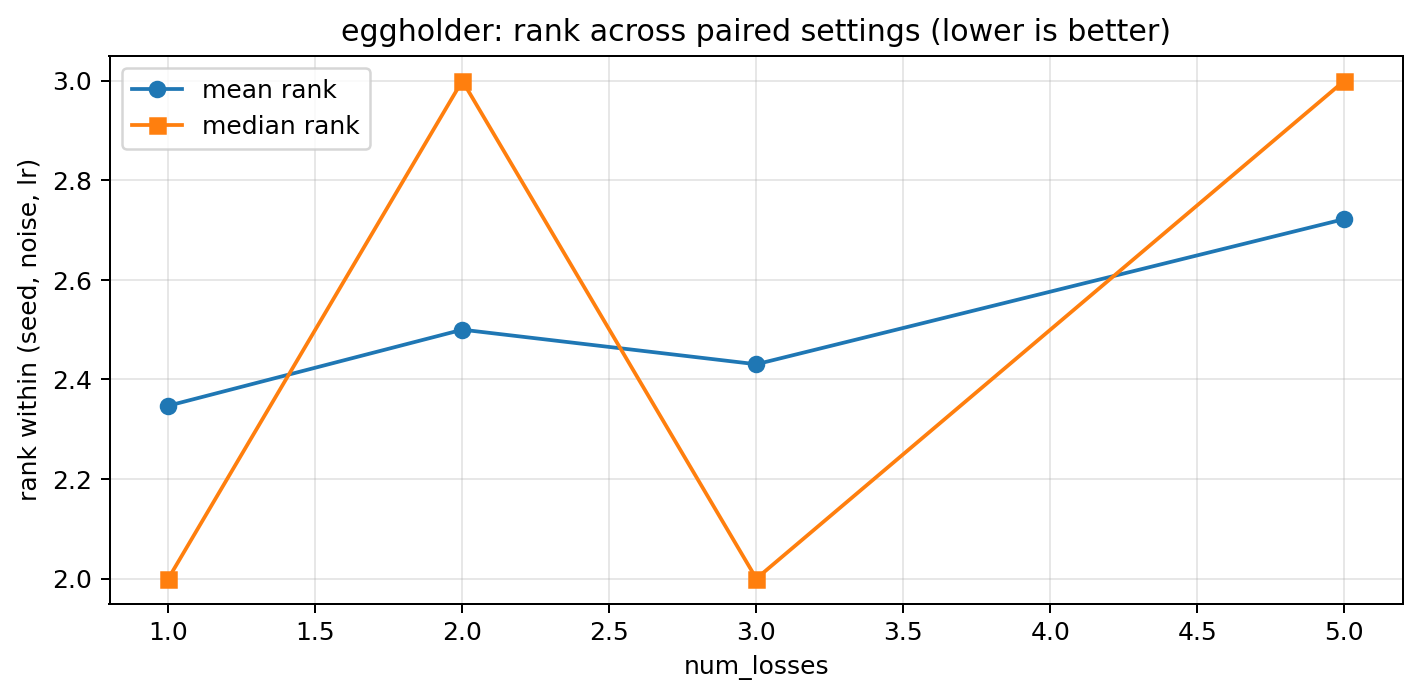
\includegraphics[width=0.72\textwidth]{figures/meta_weighting_eggholder_u1_rank_vs_num_losses.png}
    \caption{Average rank within matched settings (same seed, noise, and learning rates). Lower is better. The single-loss baseline ranks best on average, with the 3-loss setting closest behind.}
    \label{fig:meta-eggholder-u1-rank}
\end{figure}

\begin{figure}[h]
    \centering
    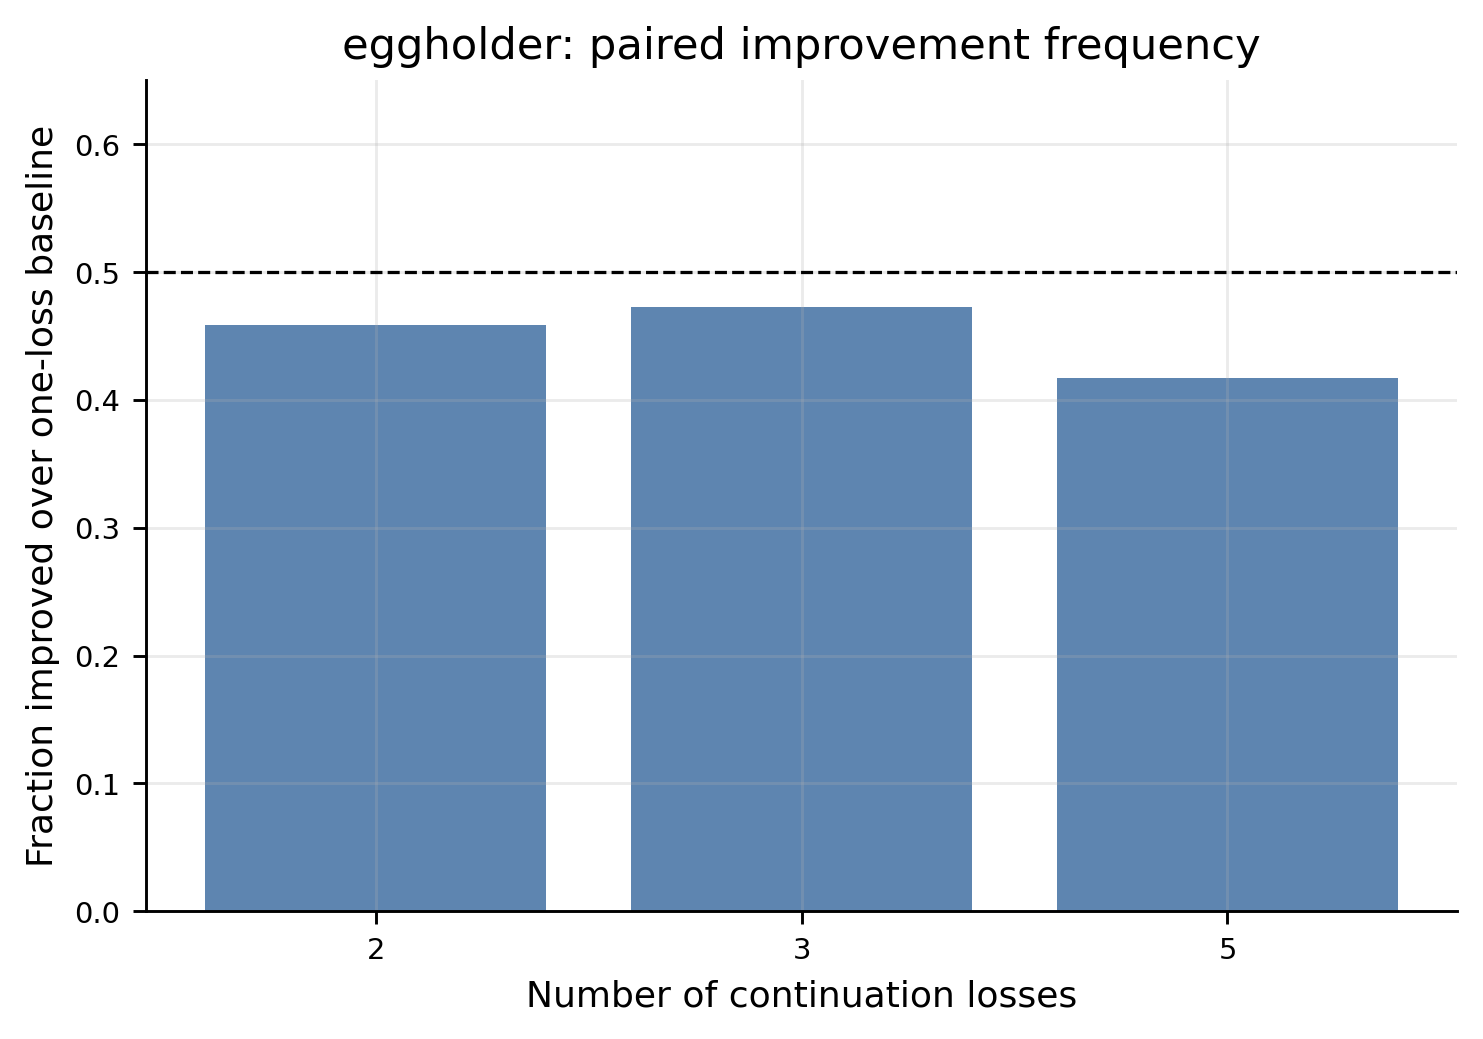
\includegraphics[width=0.72\textwidth]{figures/meta_weighting_eggholder_u1_win_rate_vs_baseline.png}
    \caption{Fraction of adaptive-weighting runs that improve over the baseline \texttt{num\_losses=1}. A value above 0.5 would indicate an advantage over the baseline. None of the adaptive settings exceed this threshold.}
    \label{fig:meta-eggholder-u1-fraction-improved}
\end{figure}

\begin{figure}[h]
    \centering
    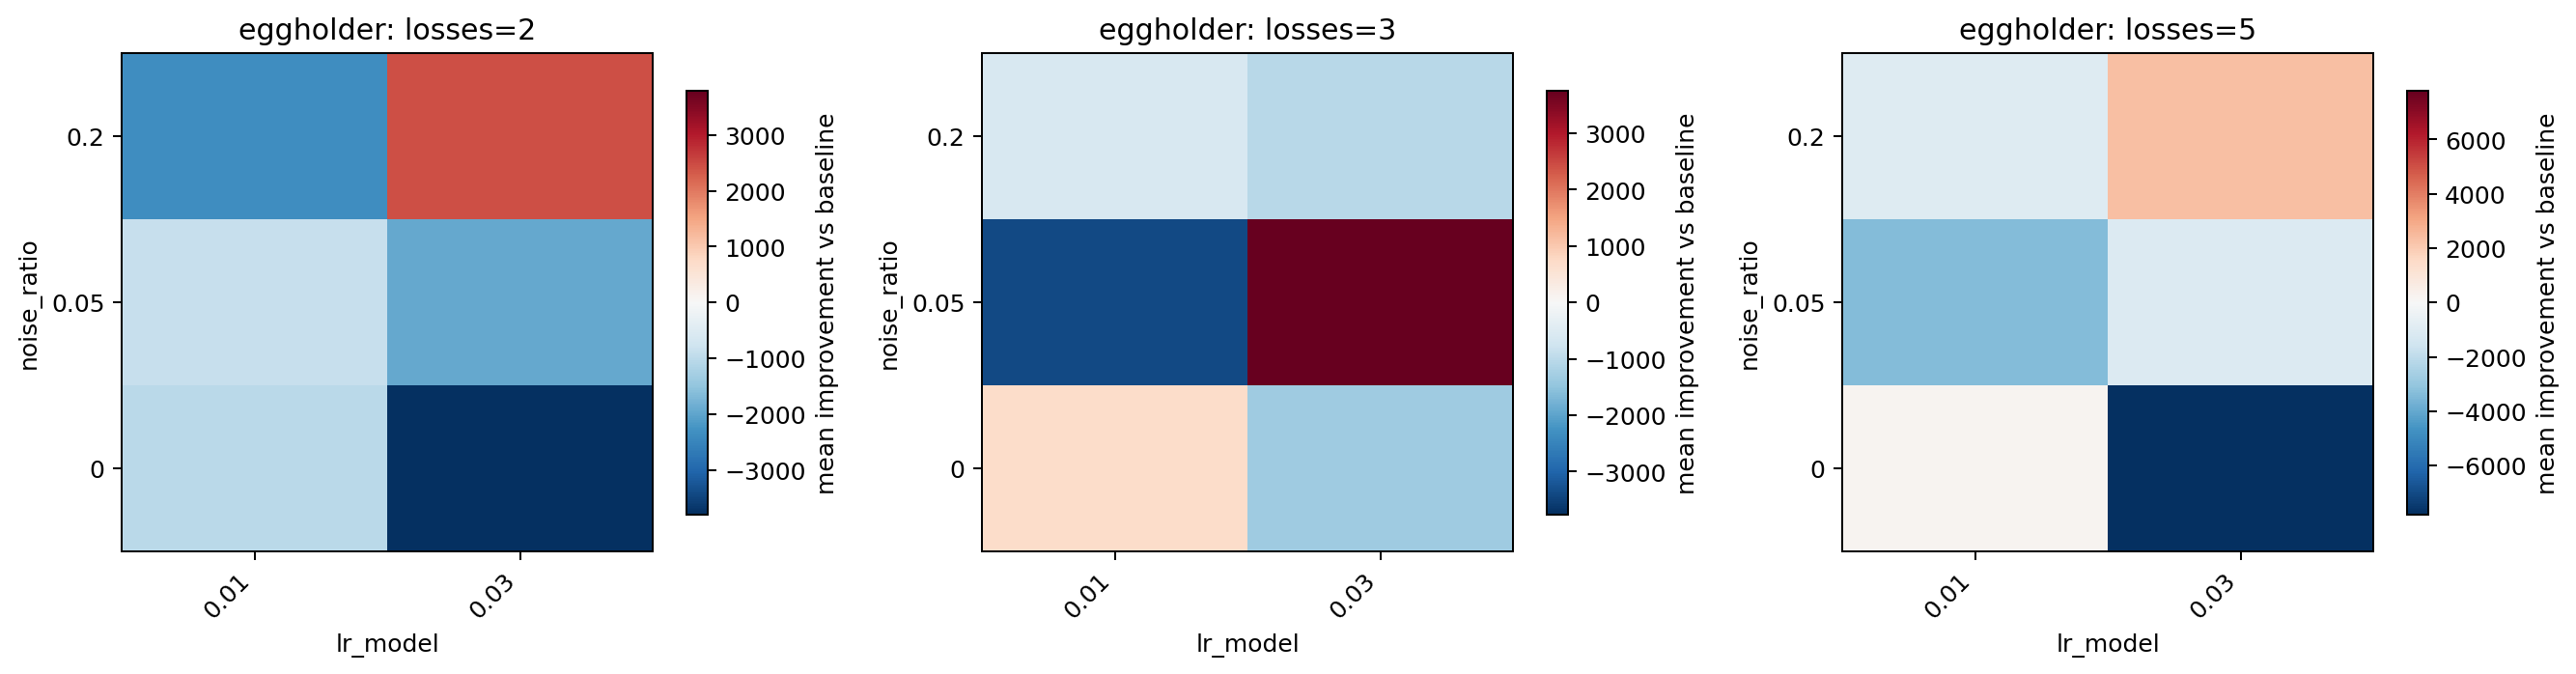
\includegraphics[width=0.88\textwidth]{figures/meta_weighting_eggholder_u1_improvement_heatmap.png}
    \caption{Mean improvement over the baseline across noise ratios and learning rates. Blue regions indicate settings where adaptive weighting improves over the baseline, while red regions indicate degradation. The pattern is mixed rather than uniformly favorable.}
    \label{fig:meta-eggholder-u1-heatmap}
\end{figure}

\section{Representative run dynamics}

To complement aggregate statistics, the next two figures show the best single
run found in the benchmark.

\begin{figure}[h]
    \centering
    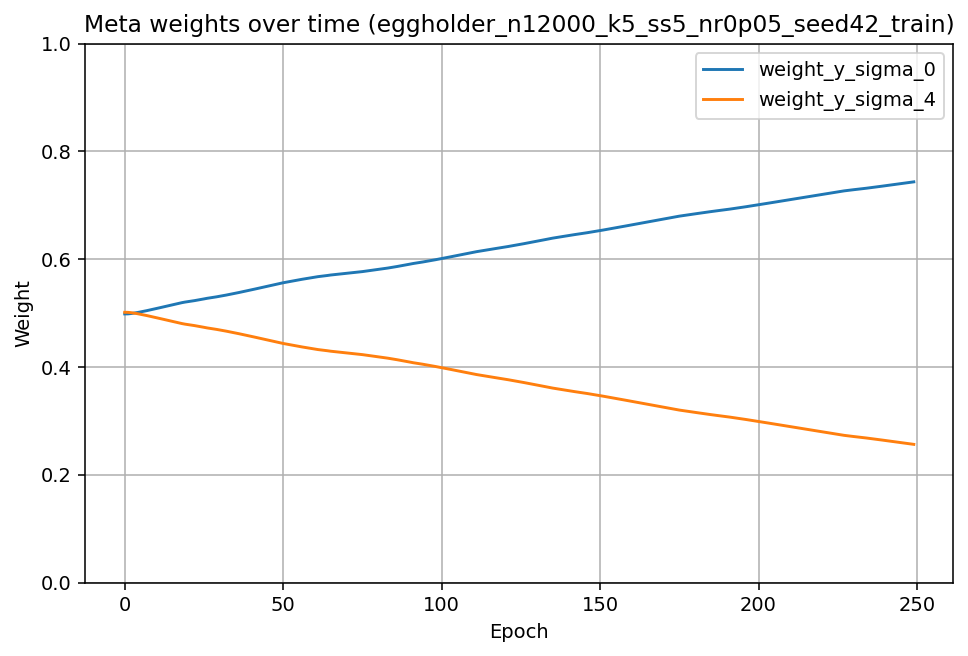
\includegraphics[width=0.82\textwidth]{figures/meta_weighting_eggholder_u1_best_weight_trajectory.png}
    \caption{Weight trajectory for the best single run (seed 42, noise 0.05, \texttt{num\_losses=2}, $\eta_{\mathrm{model}}=0.03$, $\eta_{\mathrm{meta}}=0.003$). This plot is useful for checking whether the meta-optimizer maintains a non-trivial balance between the selected losses over training.}
    \label{fig:meta-eggholder-u1-best-weights}
\end{figure}

\begin{figure}[h]
    \centering
    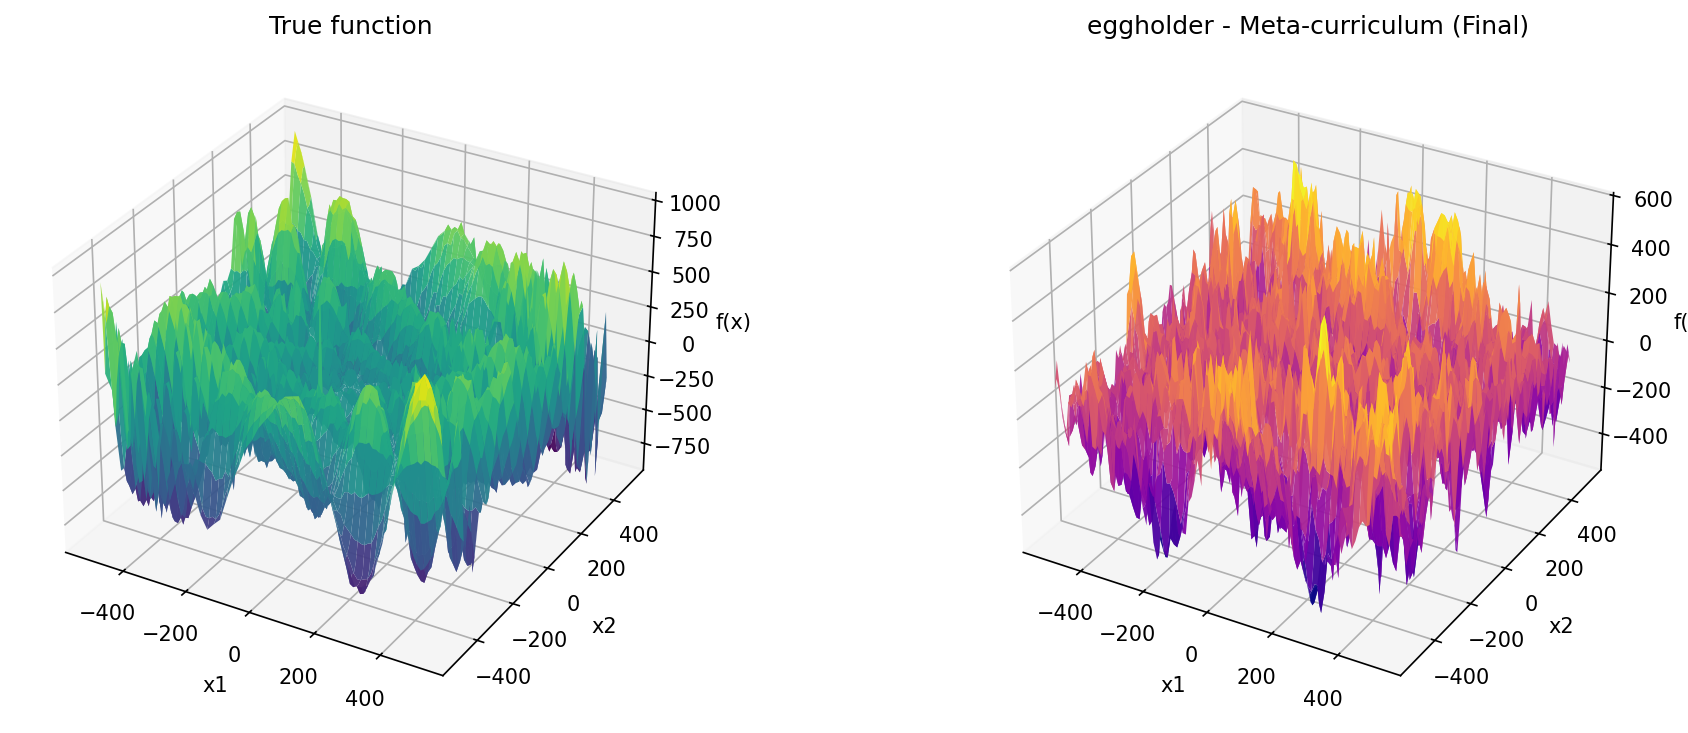
\includegraphics[width=0.78\textwidth]{figures/meta_weighting_eggholder_u1_best_final_surface.png}
    \caption{Final learned surface for the best single run according to hard validation loss.}
    \label{fig:meta-eggholder-u1-best-surface}
\end{figure}

\section{Interpretation}

\paragraph{1) Stability result.}
Restricting the meta-objective to a one-step lookahead was sufficient to make
all 288 runs complete successfully. This is an important methodological result,
because the longer unroll variants were substantially less stable in earlier
attempts.

\paragraph{2) Baseline strength.}
The single hard-target baseline remains difficult to outperform. Although adaptive
weighting sometimes finds very strong runs, its average behavior is not clearly
superior in this benchmark.

\paragraph{3) Best adaptive region.}
If adaptive weighting is pursued further for \texttt{eggholder}, the most
promising region from this benchmark appears to be:
\begin{itemize}
    \item higher model learning rate: \texttt{0.03},
    \item moderate-to-high meta learning rate: \texttt{0.001} to \texttt{0.003},
    \item a small number of losses: especially \texttt{2} or \texttt{3}.
\end{itemize}

\paragraph{4) Cost-benefit tradeoff.}
Using more weighted losses does not automatically improve the final hard-target
objective. In fact, the 5-loss setting is the most expensive conceptually and
performs worst on average in this experiment.

\section{Practical conclusion}

For the current thesis codebase and the \texttt{eggholder} benchmark,
meta-weighting with \texttt{meta\_unroll\_steps}=1 is operationally feasible and
produces interpretable weight trajectories, but it does not yet justify
replacing the direct hard-target baseline as the default method.

The most defensible conclusion at this stage is therefore:
\begin{itemize}
    \item keep \texttt{num\_losses=1} as the primary baseline,
    \item treat adaptive weighting as an exploratory extension,
    \item focus follow-up work on the narrower region where adaptive weighting
          showed occasional gains (2--3 losses, higher model LR, moderate/high
          meta LR).
\end{itemize}
